\chapter{Implemented Solution}
\section{Amazon Web Services}

\subsection{Architecture}
\begin{figure}[h]
    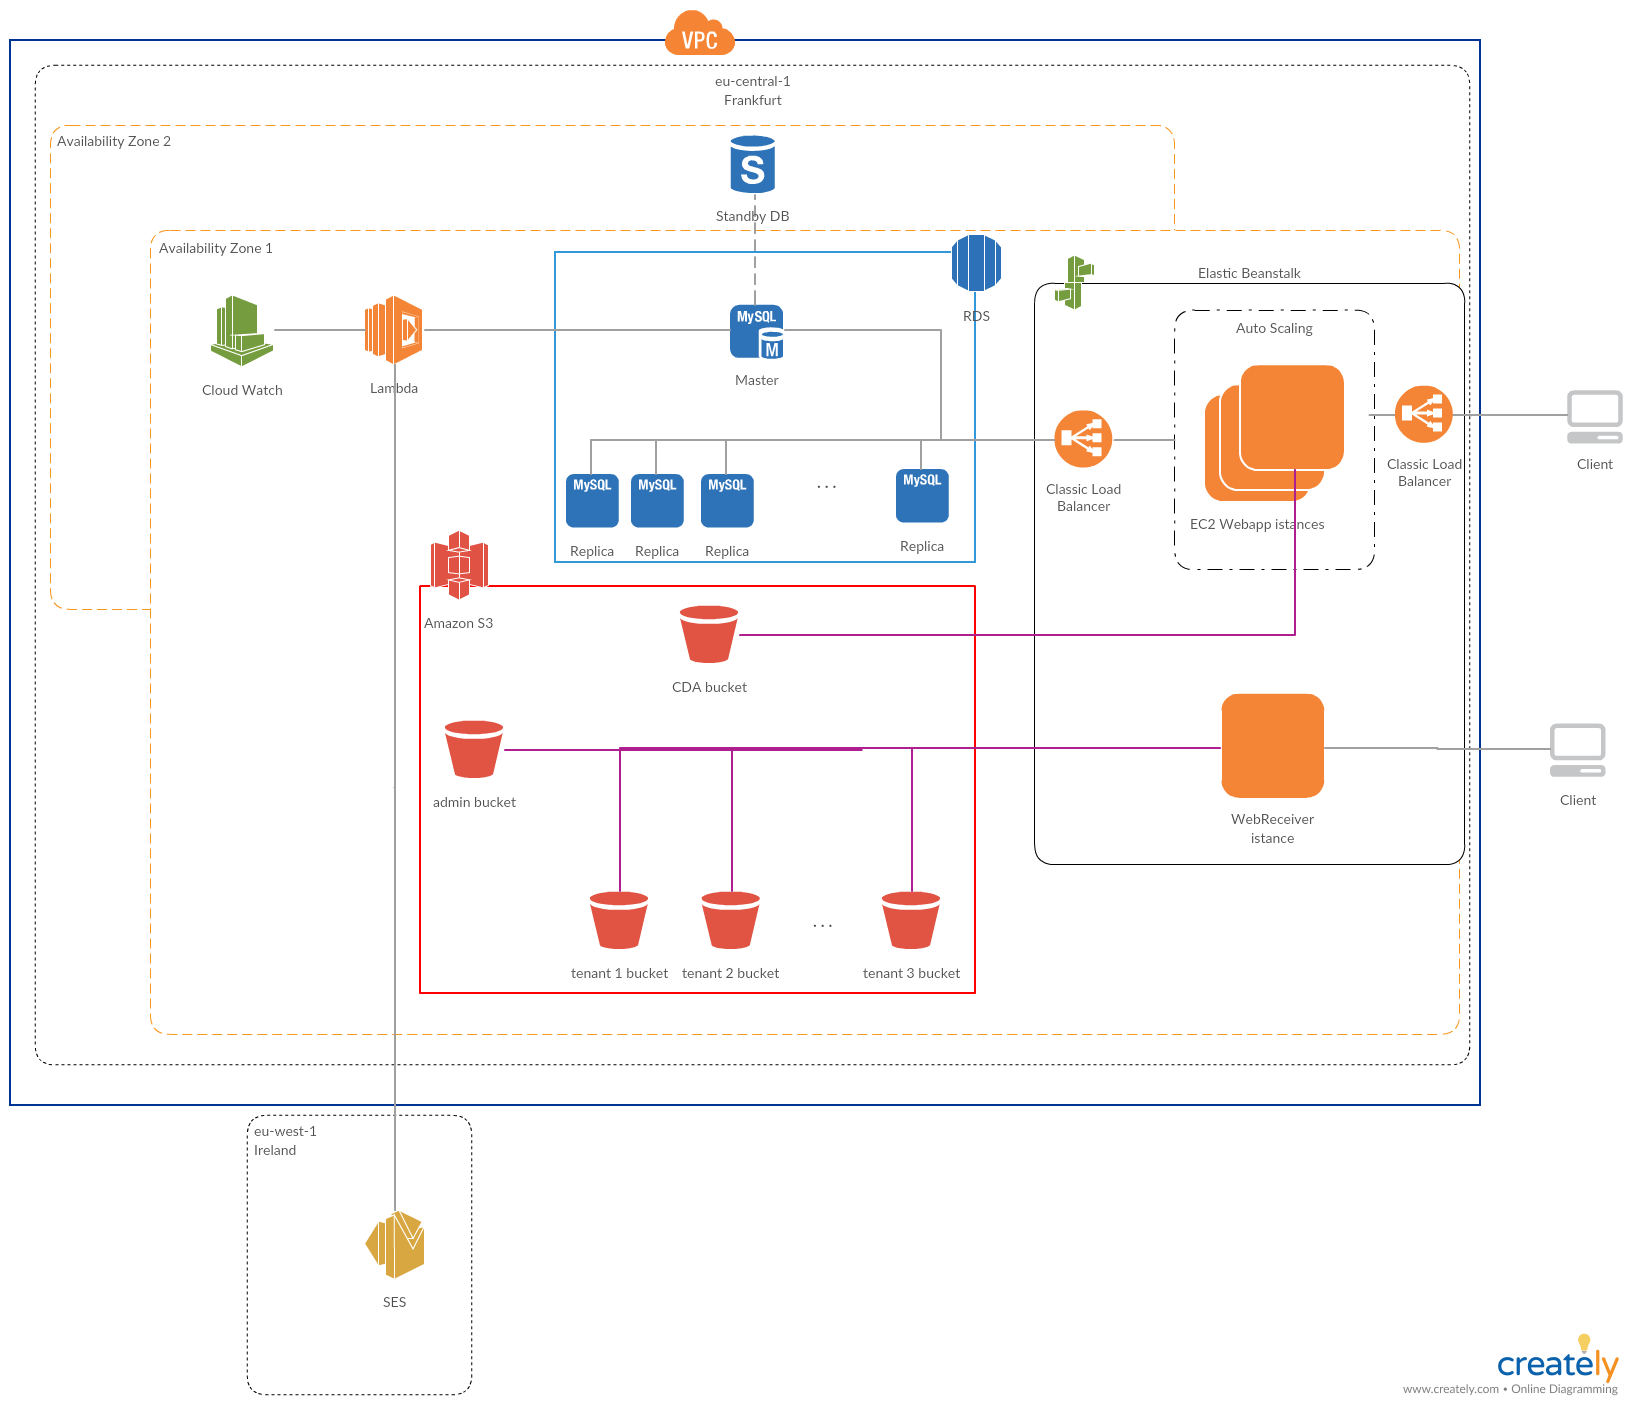
\includegraphics[width=\textwidth]{architecture}
    \caption{Architecture Scheme}
    \label{fig:architecture}
\end{figure}
Since Amazon Elastic Beanstalk (EB) has been used as the core component to manage the system, it has been possibile to use an Infrastructure as a Service grade of customization, with an easier configuration and building phase as if the system were Platform as a Service instead.\\
As shown in the picture \ref{fig:architecture}, everything but the SES service is hosted in the eu-central-1 region in Frankfurt, to reduce latency, minimize costs and keep healthcare data in an European law venue, as in production would be.
The region is divided into avaiability zones connected each other with low-latency links, so to handle potential instance failures by replacing them with the standby ones located in a different availability zone.\\
EB handles the WebServer instances: one for the EcgWebApp \ref{subsection:ecgwebapp} and the other one for WebReceiver \ref{subsection:webreceiver}, the interaction is then allowed to authenticated users bounded to their capabilities and role.\\
The persistency is achieved by a Relational Database Service (RDS) running Amazon Aurora DB, a compatible MySql Database, it is organized with a master write replica and several read replicas.
Furthermore, RDS provides a standby and synchronous Database, hosted in another availability zone, that is ready to become the new master in case of failure of the current master.\\
Furthermore all the assets and static files are read and written from/to AWS S3 relative bucket.\\
The notification System is triggered by DB events and carried on by AWS Lambda functions using Amazon Simple Email Service (SES) as delivery service to final users. The service is not available in the Frankfurt region. For this reason, the Ireland region was chosen.


\section{Ecg Workflow}
\begin{figure}[h]
    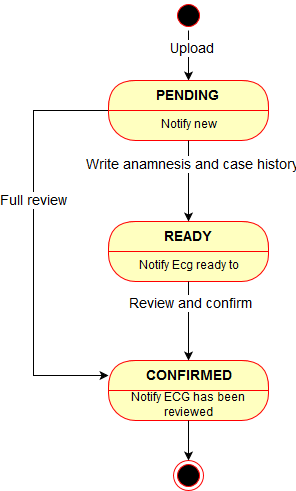
\includegraphics[width=5cm]{ECGstatechart}
    \caption{Electrocardiogram State Chart}
    \label{fig:ECGstatechart}
\end{figure}
\section{Web Applications Involved}
\subsection{EcgWebApp}
\label{subsection:ecgwebapp}
\subsection{Web Receiver}
\label{subsection:webreceiver}
\subsection{Web Uploader}
\section{S3 Bucket synchronization}
\section{Interoperability of digital electrocardiograms data}
\paragraph{Resting}
\paragraph{Cardiac stress test}
\paragraph{Holter}




